\chapter{Coordination in the Swarm}

\begin{figure} [H]

\paragraph*{}
This section talks about the lower level of robot coordination after the target object is found, and all robots surround it securely. Firstly, our robot can be controlled based on the dynamic model of an omnidirectional wheeled mobile robot. This allows our robots to obtain holonomic motion, the ability to move in the given x-y direction instantaneously without changing its pose. Hence, our team came up with a coordination method by taking advantage of holonomic constraints to plan the movements for each robot to move the target object.

\ref{fig:coordination-diagram}).

\begin{figure} [H]
    \centering
    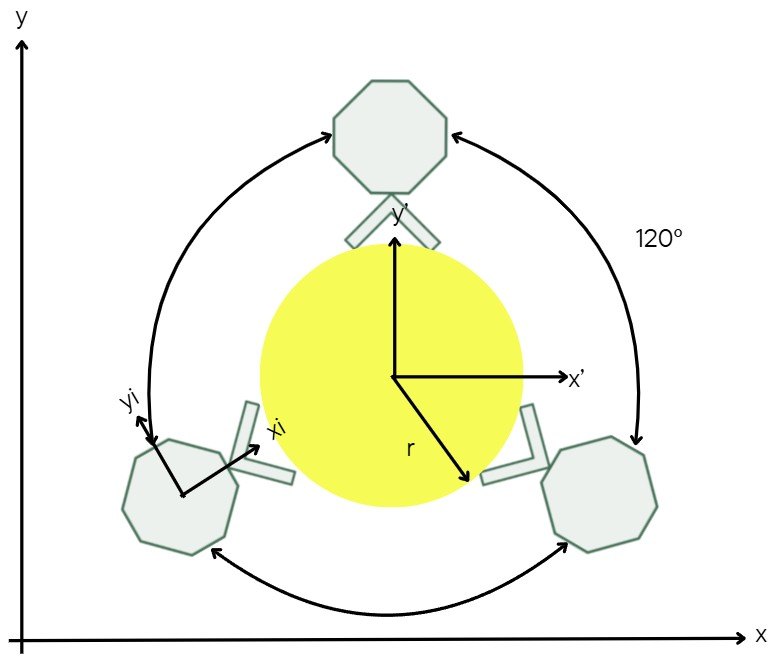
\includegraphics[width=0.5\linewidth]{assets/images/coordination/robots_with_object.jpg}
    \caption{Robots and the object in the global frame}
    \label{fig:coordination-diagram}
\end{figure}


\end{figure}
